\documentclass[12pt,a4paper,table]{article}

\usepackage{lmodern}
\usepackage[T1]{polski}
\usepackage[utf8]{inputenc}

\usepackage[a4paper,
            tmargin=2cm,
            bmargin=2cm,
            lmargin=2cm,
            rmargin=2cm,
            bindingoffset=0cm]{geometry}

\usepackage[table, w11colors]{xcolor}
\usepackage{tocloft}
\usepackage{hyperref}

\usepackage{amsmath}
\usepackage{amssymb}
\usepackage{siunitx}

\usepackage{listings}

\usepackage{graphicx}
\usepackage{subfig}
\usepackage{float}
\usepackage{booktabs}

\usepackage{tikz-timing}

\usepackage{xcolor}

% drawing state machines
\usepackage{tikz}
% \documentclass[tikz, border=2mm]{standalone}
\usepackage{karnaugh-map}
\usetikzlibrary{automata, positioning, arrows}

\tikzset{
->, % makes the edges directed
>=stealth, % makes the arrow heads bold
node distance=3cm, % specifies the minimum distance between two nodes. Change if necessary.
every state/.style={thick, fill=gray!10}, % sets the properties for each ’state’ node
initial text=$ $, % sets the text that appears on the start arrow
}



\hypersetup{
    colorlinks,
    citecolor=black,
    filecolor=black,
    linkcolor=black,
    urlcolor=black
}

\newtheorem{definition}{Def}


\begin{document}
    \title {
        Technika Cyfrowa - Sprawozdanie nr 3
    }

    \author{
        Jan Chyczyński \\
        Błażej Nowicki \\
        Bartłomiej Słupik \\
        Przemysław Węglik
    }

    \date{\today}

    \maketitle

    \section{Zadanie 3a}
    Zadanie polega na zaprojektowaniu i przetestowaniu dwójki logicznej w oparciu
    o przerzutnik JK. Następnie należy zastosować zaprojektowany układ w budowie 
    asynchronicznego licznika modulo 8.

    \subsection{Idea}
    \subsubsection{Dwójka licząca}
    Dwójka licząca to układ, który posiada wejście zegarowe CLK i wyjście Q. Przy kolejnych
    impulsach zegara, a dokładniej przy przejściu ze stanu niskiego na wysoki,
    stan wyjścia Q jest zmieniany na przeciwny.

    \begin{figure}[H]
        \centering
        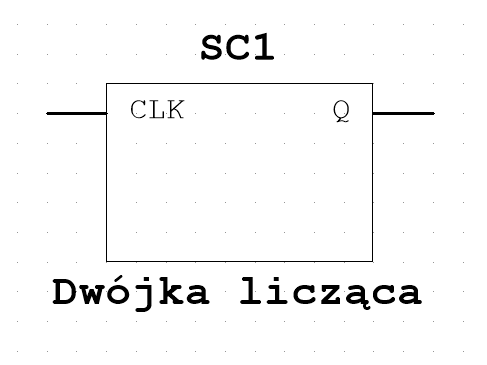
\includegraphics[width=1\linewidth]{images/dwojka_liczaca.PNG}
        \caption{Schemat koncepcyjny dwójki liczącej}
        \label{fig:dwojka_koncepcja}
    \end{figure}

    \begin{table}[h]
        \centering
        \begin{tabular}{|c|c|}
            \hline
            Q & $Q_+$ \texttiming{LH} \\ \hline
            1 & 0 \\ \hline
            0 & 1 \\ \hline
        \end{tabular}
        \caption{Oczekiwana tabela prawdy układu. Spełnia on równanie $Q_+ = \overline{Q}$}
        \label{tab:dwojka_truthtable}
    \end{table}


    \pagebreak
    \subsection{Rozwiązanie teoretyczne}
    \subsubsection{Dwójka licząca}
    \label{solution}
    W implementacji dwójki liczącej należało użyć przerzutnika typu JK. Poniżej przedstawiono
    tabelę prawdy tego przerzutnika:

    \begin{table}[h]
        \centering
        \begin{tabular}{|ccc|c|}
            \hline
            J & K & Q & $Q_+$ \texttiming{LH} \\ \hline
            0 & 0 & 0 & 0 \\
            0 & 0 & 1 & 1 \\
            \rowcolor{cyan}
            1 & 0 & 0 & 1 \\
            1 & 0 & 1 & 1 \\
            0 & 1 & 0 & 0 \\
            \rowcolor{lime}
            0 & 1 & 1 & 0 \\
            \rowcolor{cyan}
            1 & 1 & 0 & 1 \\
            \rowcolor{lime}   
            1 & 1 & 1 & 0 \\ \hline        
        \end{tabular}
        \caption{Tabela prawdy przerzutnika JK. \\Kolor niebieski to przejście $Q$ z 0 na 1, zielony - z 1 na 0}
        \label{tab:JK_truthtable}
    \end{table}

    Szukamy funkcji J(Q) i K(Q), która spełnia warunek $Q_+ = \overline{Q}$.
    Warunek zachodzi dla każdej kombinacji wierszy zielonych z niebieskimi.
    To znaczy, że rozwiązaniami są:
    \begin{enumerate}
        \item $J(Q) = \overline{Q},\; K(Q) = Q$ (wiersz 3. i 6.)
        \item $J(Q) = 1,\; K(Q) = Q$ (wiersz 3. i 8.)
        \item $J(Q) = \overline{Q},\; K(Q) = 1$ (wiersz 7. i 6.)
        \item $J(Q) = 1,\; K(Q) = 1$ (wiersz 7. i 8.)
    \end{enumerate}

    
    Rozwiązanie korzystające z wierszy 7. i 8. jest znacznie prostsze w implementacji,
    gdyż wymaga tylko podłączenia J i K wysoko.  Zatem schemat układu może wyglądać tak, jak na poniższym rysunku:

    \begin{figure}[H]
        \centering
        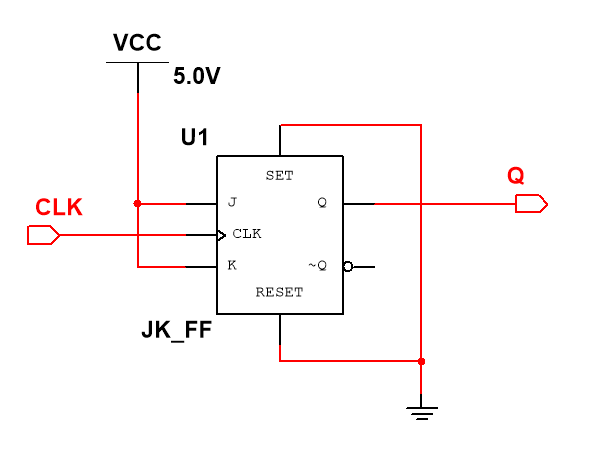
\includegraphics[width=0.7\linewidth]{images/dwojka_schemat.PNG}
        \caption{Schemat układu dwójki liczącej}
        \label{fig:dwojka_schemat}
    \end{figure}


    \pagebreak
    \subsection{Symulacja w programie Multisim}
    \subsubsection{Dwójka licząca}
    W programie Multisim stworzono następujący układ testowy składający się ze źródła fali
    prostokątnej, dwójki liczącej, generatora słów binarnych oraz analizatora stanów logicznych:

    \begin{figure}[h]
        \centering
        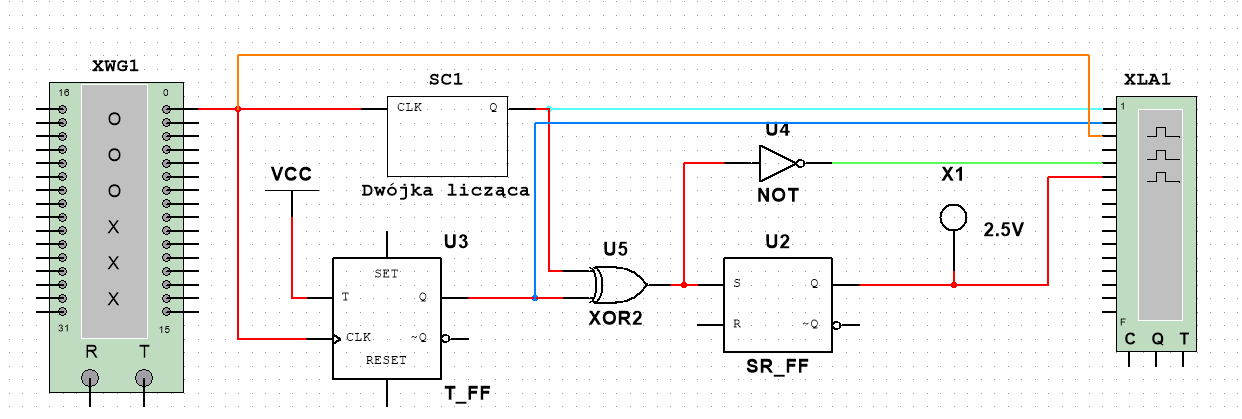
\includegraphics[width=1\linewidth]{images/dwojka_test.PNG}
        \caption{Schemat układu testującego}
        \label{fig:dwojka_test}
    \end{figure}

    \begin{figure}[h]
        \centering
        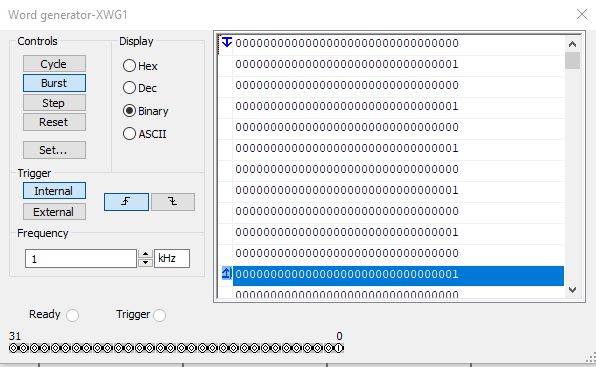
\includegraphics[width=1\linewidth]{images/dwojka_xwg.PNG}
        \caption{Stan generatora słów}
        \label{fig:dwojka_xwg}
    \end{figure}

    Przeprowadzono symulację i uzyskano następujące dane na analizatorze:

    \begin{figure}[H]
        \centering
        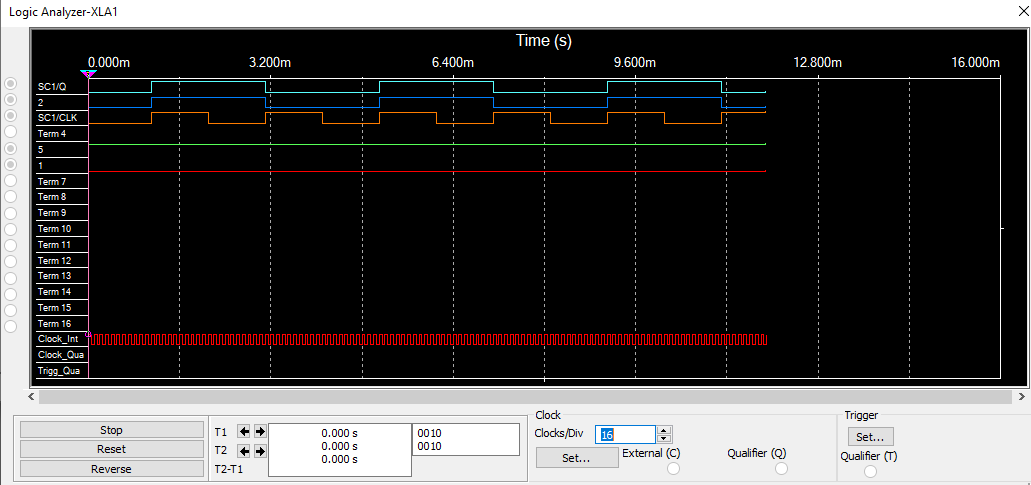
\includegraphics[width=\linewidth]{images/dwojka_xla.PNG}
        \caption{Wykresy stanów na ekranie analizatora}
        \label{fig:dwojka_xla}
    \end{figure}

    Widać, że oczekiwany efekt zachodzi - wyjście Q zmienia stan na przeciwny przy impulsie zegara.
    Fala na wyjściu ma dwukrotnie większy okres, niż ta na wejściu.

    \subsection{Zastosowania}
    \begin{enumerate}
        \item Dwójkę liczącą można zastosować do 
        dwukrotnego zmniejszenia częstotliwości fali
        prostokątnej.

        \item Dwójkę liczącą można zastosować również w 
        sterowaniu innymi układami przy pomocy
        przycisku dzwonkowego, aby uzyskać dwa ciągłe 
        stany i przełączać się między nimi przy
        kolejnych naciśnięciach - na przykład włączanie 
        i wyłączanie lampy.

        \item Dwójkę liczącą można zastosować także na linii produkcyjnej, jeśli chcemy rozdzielić
        obróbkę produktu na dwie maszyny. Dzięki dwójce liczącej możemy podawać sygnał
        raz na jedną raz na drugą maszynę.
    \end{enumerate}

    \subsection{Wnioski}
    \begin{enumerate}
        \item Dwójkę liczącą można zaimplementować także na inne 
        sposoby wynikające z tabeli prawdy
        (\hyperref[tab:JK_truthtable]{Tabela \ref{tab:JK_truthtable}}).
        W praktyce jednak wybraliśmy najprostyszy do skonstruowania.
    \end{enumerate}

    \subsection{Idea}
    \subsubsection{Licznik modulo 8}
    Licznik modulo 8 to układ, który posiada wejście zegarowe CLK i 
    wyjścia $Q_0$, $Q_1$, $Q_2$. Przy kolejnych
    impulsach zegara, a dokładniej przy przejściu ze stanu niskiego na wysoki,
    stan wyjścia zmieniany jest na kolejną liczbę binarną. Układ liczy do 7 w systemie
    dwójkowym, a potem wraca do 0.

    \begin{figure}[H]
        \centering
        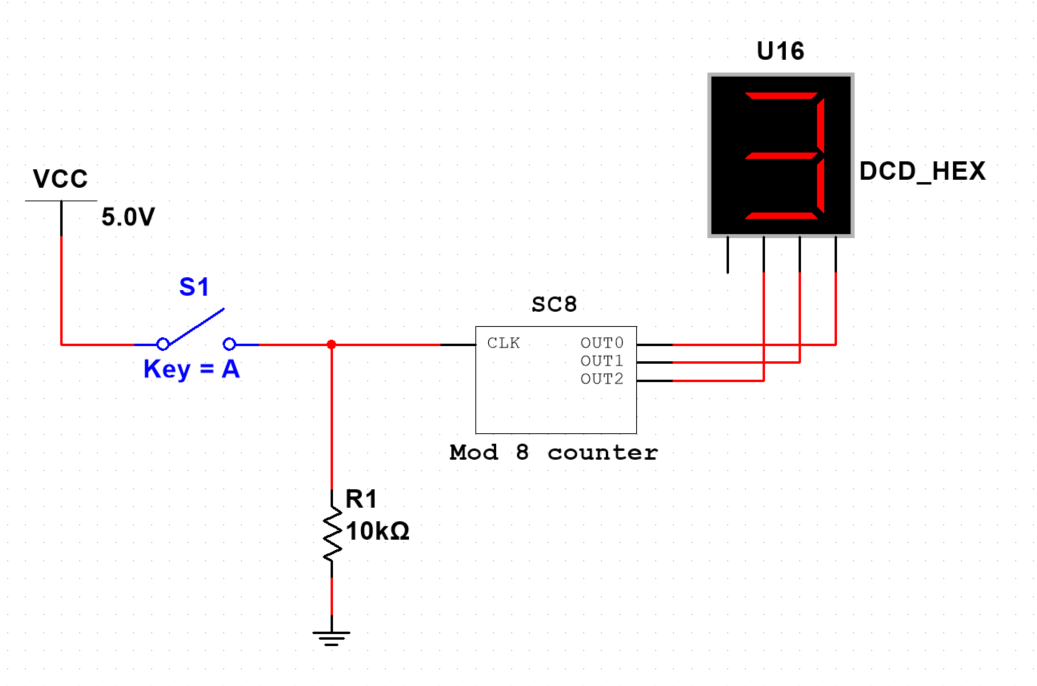
\includegraphics[width=1\linewidth]{images/mod8_idea.PNG}
        \caption{Schemat koncepcyjny licznika modulo 8}
        \label{fig:mod8_koncepcja}
    \end{figure}

    \begin{table}[h]
        \centering
        \begin{tabular}{|ccc|ccc|}
            \hline
            $Q_0$ & $Q_1$ & $Q_2$ & $Q_0+$ & $Q_1+$ & $Q_2+$ \\
            \hline
            0 & 0 & 0 & 0 & 0 & 1\\
            0 & 0 & 1 & 0 & 1 & 0\\ 
            0 & 1 & 0 & 0 & 1 & 1\\
            0 & 1 & 1 & 1 & 0 & 0\\ 
            1 & 0 & 0 & 1 & 0 & 1\\
            1 & 0 & 1 & 1 & 1 & 0\\ 
            1 & 1 & 0 & 1 & 1 & 1\\
            1 & 1 & 1 & 0 & 0 & 0\\ 
            \hline
        \end{tabular}
        \caption{Tabela przedstawiające kolejne przejścia licznika modulo 8}
        \label{tab:mod8_truthtable}
    \end{table}

    \subsection{Rozwiązanie teoretyczne}
    \subsubsection{Licznik modulo 8}
    Zauważmy, że najmłodszy bit zmienia swój stan w każdym takcie zegara, a $n+1$ -szy 
    zmienia się tylko wtedy gdy na $n$-tym bicie następuje przeniesienie (zmiana z 1 na 0). 
    Oddaje
    to naturę liczenia w systemie binarnym.
    (\hyperref[tab:mod8_truthtable]{Patrz tabela \ref{tab:mod8_truthtable}}).
    Oznacza to, że do implementacji licznika modulo 8 można użyć 3 dwójek liczących, gdzie
    każda dwójka reprezentuje jeden bit liczby 3-bitowej. 
    Ponieważ nasze dwójki liczące zmieniają stan przy wzroście sygnału wejściowego (zmiana z 0 na 1)
    to wsytarczy połączyć kolejne dwójki bramkami NOT
    A zatem schemat takiego układu może wygladać jak poniżej:
    \begin{figure}[H]
        \centering
        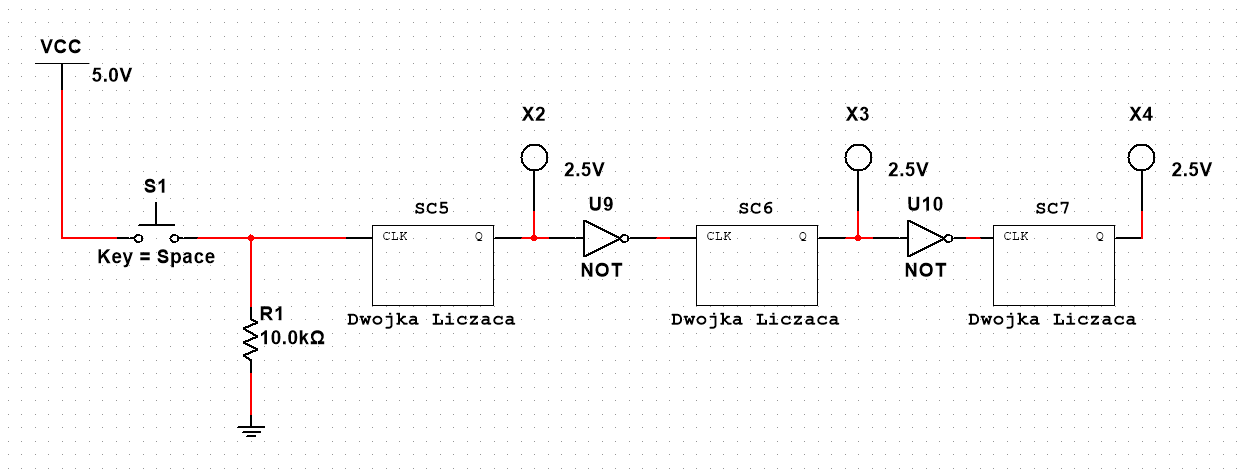
\includegraphics[width=1.05\linewidth]{images/mod8_schematic.PNG}
        \caption{Schemat układu licznika modulo 8}
        \label{fig:mod8_schemat}
    \end{figure}

    \subsection{Implementacja w programie Multisim}
    \subsubsection{Licznik modulo 8}

    \begin{figure}[h]
        \centering
        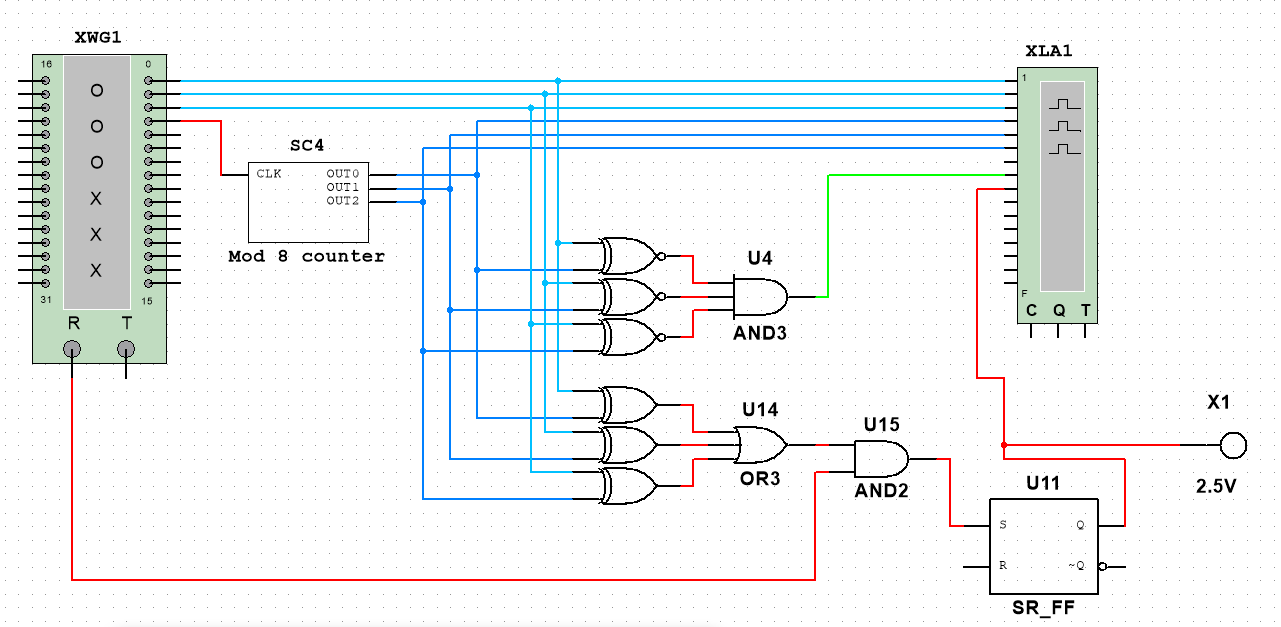
\includegraphics[width=1\linewidth]{images/mod8_testy.PNG}
        \caption{Schemat układu testującego}
        \label{fig:mod8_testy}
    \end{figure}

    \begin{figure}[h]
        \centering
        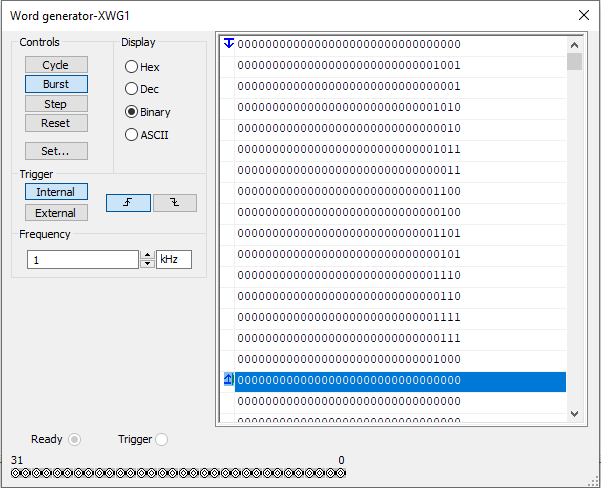
\includegraphics[width=1\linewidth]{images/mod8_xwg.PNG}
        \caption{Stan generatora słów}
        \label{fig:mod8_xwg}
    \end{figure}
    Przeprowadzono symulację i uzyskano następujące dane na analizatorze:

    \begin{figure}[H]
        \centering
        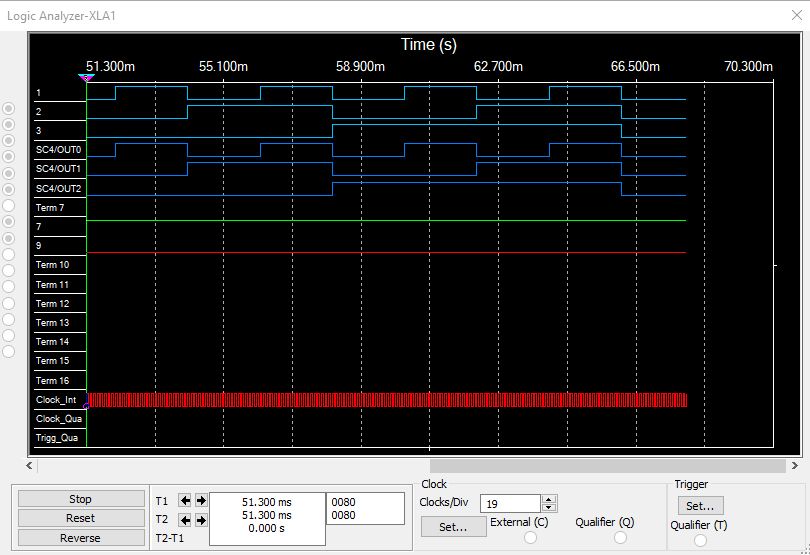
\includegraphics[width=\linewidth]{images/mod8_xla.PNG}
        \caption{Wykresy stanów na ekranie analizatora}
        \label{fig:mod8_xla}
    \end{figure}

    \subsection{Zastosowania}
    \begin{enumerate}
        \item Licznik modulo 8 możemy wykorzystać w oprogramowaniu wiatraka chłodzącego pokój.
        Śmigła wiatraka przyczepione są do serwomechanizmu, do którego podajemy kolejne liczby z licznika.
        Liczby wskazują kolejne pozycje serwa.

        \item Robot przemysłowy posiadajacy 8 możliwych stanów. Jego aktualna 
        pozycja jest definiowana wyjściem z licznika modulo 8.

        \item Poziom ciepła w płycie grzewczej. Kiedy klikamy klawisz zmiany
        temperatury, licznik inkrementuje się zmieniając temperaturę kuchenki.
    \end{enumerate}

    \pagebreak
    \section{Zadanie 3b}
    Zadanie polega na zaprojektowaniu i zbudowaniu synchronicznego czterobitowego licznika
    liczącego w kodzie Gray'a.

    \subsection{Idea}
    Układ docelowy powinien posiadać wejście zegara CLK oraz cztery wyjścia
    $Q_1, Q_2, Q_3, Q_4$ odwzorowywujące cyfry czterobitowej liczby zapisanej w kodzie Gray'a.
    Przy impulsie zegara, wyjście powinno przestawiać się na kolejną liczbę, a z ostatniego
    stanu $1111_2 = 1000_Q$ wrócić na początkowy - $0000_2 = 0000_Q$.

    \begin{figure}[h]
        \centering
        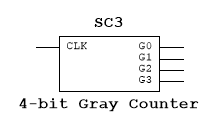
\includegraphics[width=\linewidth]{images/gray_idea.PNG}
        \caption{Schemat koncepcyjny licznika w kodzie Gray'a}
        \label{fig:gray_idea}
    \end{figure}

    \begin{table}[h]
        \centering
        \begin{tabular}{|cc|cc|cc|cc|}
            \hline
            $n$ & $Q_3Q_2Q_1Q_0 $ & $n$ & $Q_3Q_2Q_1Q_0 $ & $n$ & $Q_3Q_2Q_1Q_0 $ & $n$ & $Q_3Q_2Q_1Q_0 $ \\
            \hline
            0 & 0000 & 4 & 0110 & 8  & 1100 & 12 & 1010 \\
            1 & 0001 & 5 & 0111 & 9  & 1101 & 13 & 1011 \\
            2 & 0011 & 6 & 0101 & 10 & 1111 & 14 & 1001 \\
            3 & 0010 & 7 & 0100 & 11 & 1110 & 15 & 1000 \\
            \hline
        \end{tabular}
        \caption{Oczekiwane wyjścia układu dla kolejnych stanów}
        \label{tab:gray_exp_output}
    \end{table}

    \pagebreak
    \subsection{Rozwiązanie teoretyczne}
    \subsubsection{Tabela prawdy układu}
    Jako, że układ ma 16 możliwych stanów, można zaprojektować go na czterech przerzutnikach. 
    Zdecydowaliśmy się na przerzutniki T, gdyż kod Gray'a bazuje na zmianach stanu jednego, danego bitu.
    Układ posiada 8 zmiennych: wyjścia przerzutników $Q_3, \dots, Q_0$ i ich wejścia T: $T_3, \dots, T_0$.
    Oczekiwane stany tych zmiennych przedstawiono w Tabeli \ref{tab:gray_states}.

    \begin{table}[h]
        \centering
        \begin{tabular}{|c|cccc|c|cccc|} 
            \hline
            N & $Q_3$ & $Q_2$ & $Q_1$ & $Q_0$ & Zmiana & $T_3$ & $T_2$ & $T_1$ & $T_0$ \\ \hline
            0&	0&	0&	0&	0&	0 $\rightarrow$ 1&	    0&	0&	0&	1 \\
            1&	0&	0&	0&	1&	1 $\rightarrow$ 2&	    0&	0&	1&	0 \\
            2&	0&	0&	1&	1&	2 $\rightarrow$ 3&	    0&	0&	0&	1 \\
            3&	0&	0&	1&	0&	3 $\rightarrow$ 4&	    0&	1&	0&	0 \\
            4&	0&	1&	1&	0&	4 $\rightarrow$ 5&	    0&	0&	0&	1 \\
            5&	0&	1&	1&	1&	5 $\rightarrow$ 6&	    0&	0&	1&	0 \\
            6&	0&	1&	0&	1&	6 $\rightarrow$ 7&	    0&	0&	0&	1 \\
            7&	0&	1&	0&	0&	7 $\rightarrow$ 8&	    1&	0&	0&	0 \\
            8&	1&	1&	0&	0&	8 $\rightarrow$ 9&	    0&	0&	0&	1 \\
            9&	1&	1&	0&	1&	9 $\rightarrow$ 10&    0&	0&	1&	0 \\
            10&	1&	1&	1&	1&	10 $\rightarrow$ 11&	0&	0&	0&	1 \\
            11&	1&	1&	1&	0&	11 $\rightarrow$ 12&	0&	1&	0&	0 \\
            12&	1&	0&	1&	0&	12 $\rightarrow$ 13&	0&	0&	0&	1 \\
            13&	1&	0&	1&	1&	13 $\rightarrow$ 14&	0&	0&	1&	0 \\
            14&	1&	0&  0&	1&	14 $\rightarrow$ 15&	0&	0&	0&	1 \\
            15&	1&	0&	0&	0&	15 $\rightarrow$ 0&    1&	0&	0&	0 \\
            \hline
        \end{tabular}
        \caption{Oczekiwane stany zmiennych układu}
        \label{tab:gray_states}
    \end{table}
    
    \subsubsection{Wyprowadzenie funkcji logicznych}
    Stosując tabele Karnough przedstawione \textbf{na kolejnej stronie}, wyprowadzono wzory na $T_0, \dots, T_3$ 
    (wykorzystujemy to, że zanegowany $XOR$ to równoważność):
    \begin{align*}
        T_0 &= \overline{(Q_1 \oplus Q_3) \cdot (Q_0 \oplus Q_2)} \\
        T_1 &= Q_0 \cdot \overline{(Q_3 \oplus (Q_1 \oplus Q_2))} \\
        T_2 &= Q_1 \cdot \overline{Q_0} \cdot \overline{(Q_3 \cdot Q_2)} \\
        T_3 &= \overline{Q_0} \cdot \overline{Q_1} \cdot (Q_3 \oplus Q_2)
    \end{align*}
    

    \begin{figure}[hp]
        \centering
        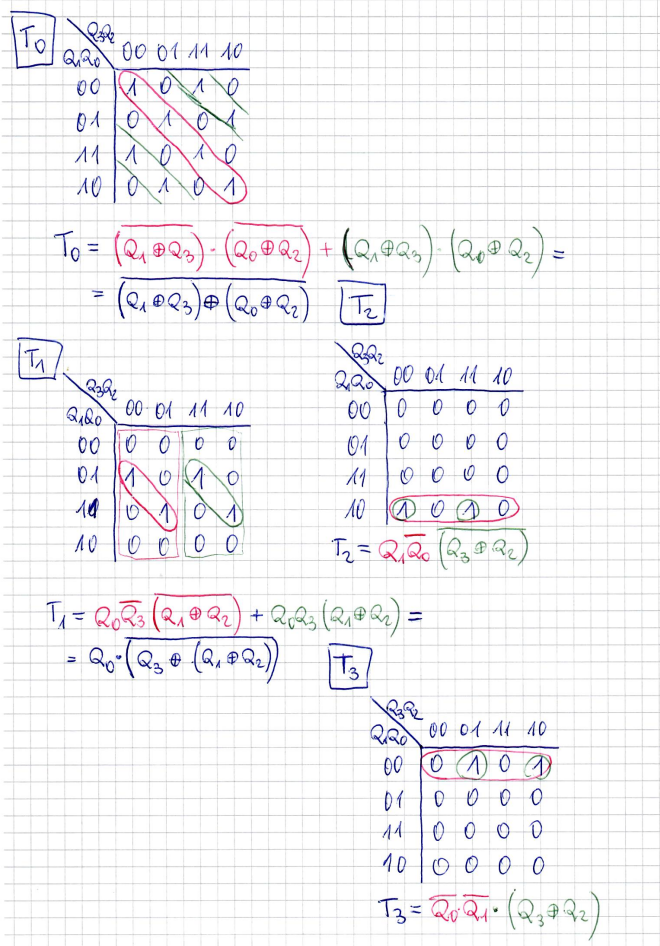
\includegraphics[width=\linewidth]{images/gray_wyprowadzenie.PNG}
        \caption{Wyprowadzenie funkcji $T_0, \dots T_3$ przy pomocy tabeli Karnough}
    \end{figure}


    \pagebreak
    \subsubsection{Schemat czterobitowego licznika Gray'a}
    Po podłączeniu wszystkich wejść $T_i$ według planu, otrzymujemy następujący schemat:
    \begin{figure}[h]
        \centering
        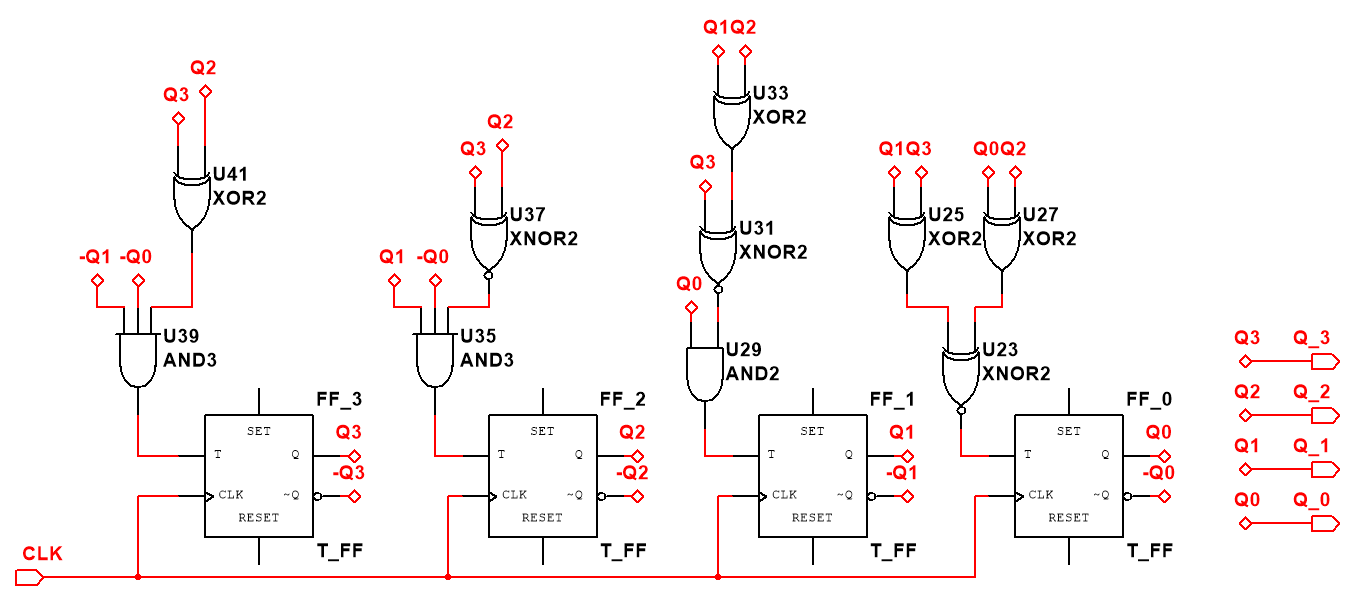
\includegraphics[width=1.1\linewidth]{images/gray_schematic.PNG}
        \caption{Schemat czterobitowego licznika liczącego w kodzie Gray'a}
        \label{fig:gray_schemat}
    \end{figure}

    \subsection{Testy w programie Multisim}
    W programie Multisim stworzono następujący układ testowy, składający się z badanego układu, 
    generatora fali prostokątnej, generatora słów binarnych oraz analizatora logicznego. Logika
    ma na celu stwierdzenie równoważności wyjścia oczekiwanego i otrzymanego.
    \begin{figure}[h]
        \centering
        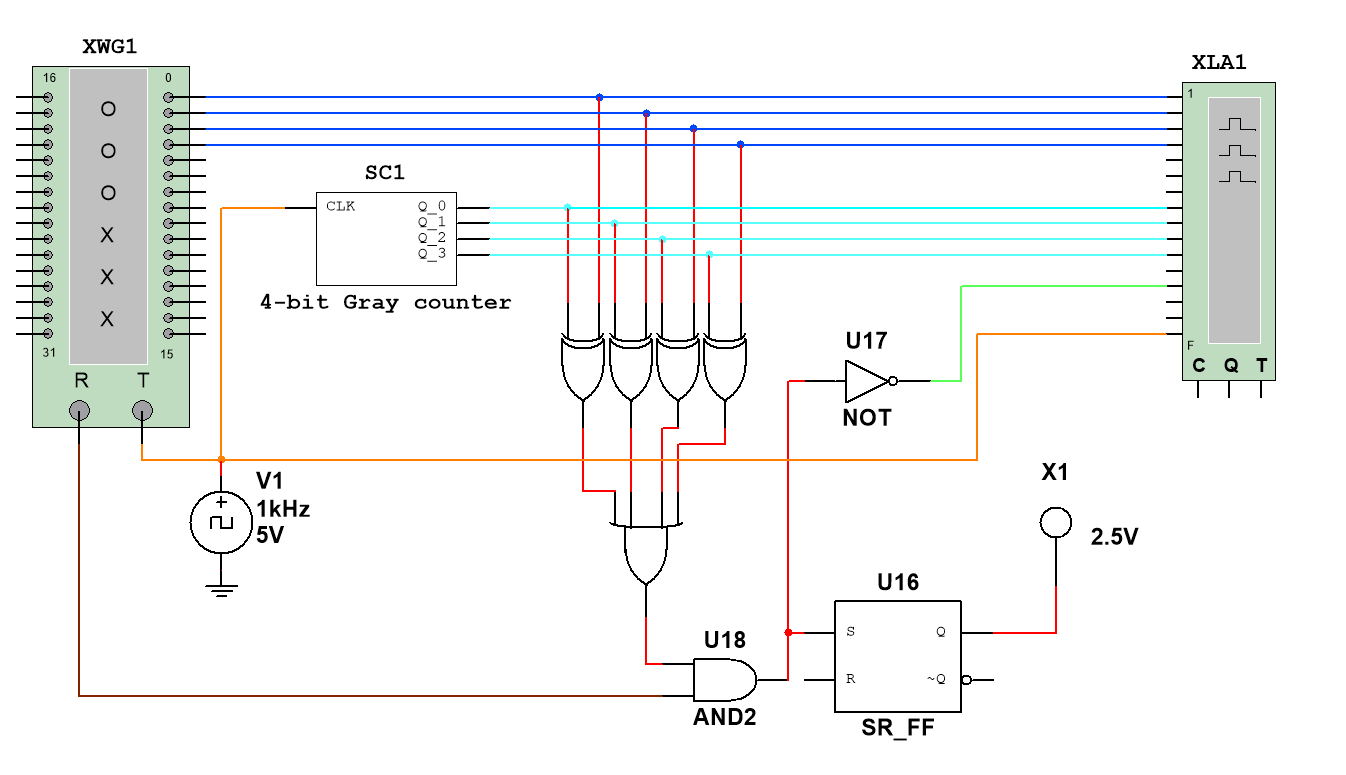
\includegraphics[width=\linewidth]{images/gray_test.PNG}
        \caption{Schemat układu testującego}
        \label{fig:gray_test}
    \end{figure}

    \pagebreak
    W generatorze słów binarnych wpisano liczby z zakresu 0-15 w kodzie Gray'a:
    \begin{figure}[h!]
        \centering
        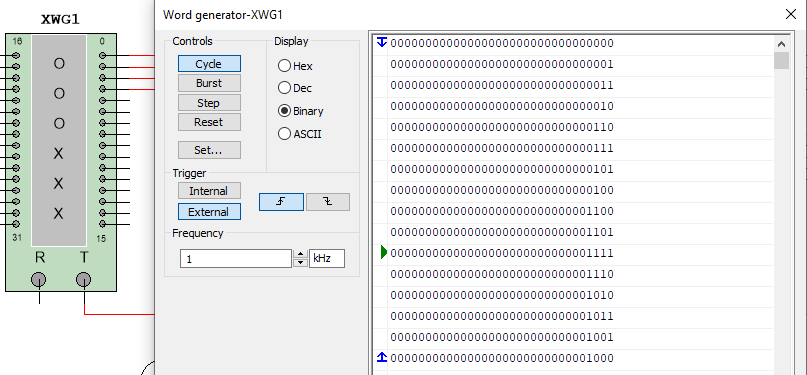
\includegraphics[width=0.8\linewidth]{images/gray_xwb.PNG}
        \caption{Ustawienia generatora słów binarnych}
        \label{fig:gray_xwb}
    \end{figure}

    Poniżej przedstawiono wykres wygenerowany przez analizator stanów logicznych:
    \begin{figure}[H]
        \centering
        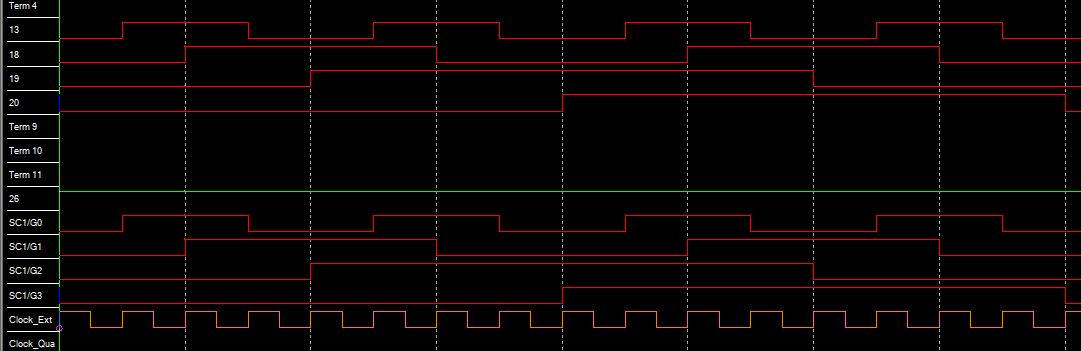
\includegraphics[width=0.9\linewidth]{images/gray_xla.PNG}
        \caption{Przebieg stanów logicznych podczas 16 cykli zegara}
        \label{fig:gray_xla}
    \end{figure}

    Górne wykresy to wyjście oczekiwane, dolne - wyjście uzyskane. Zielony wykres to równoważność
    tych stanów - jest zawsze w stanie wysokim, co dowodzi poprawności działania układu
    \pagebreak
    \subsection{Wnioski}
    \begin{enumerate}
        \item Licznik w kodzie Gray'a ma przewagę nad zwykłym licznikiem binarnym, gdyż podczas przejścia
        między kolejnymi stanami zmienia się tylko jeden bit. Odczytując jego wartość podczas tranzycji
        pomylimy się maksymalnie o 1.
    \end{enumerate}

    \subsection{Zastosowania}
    \begin{enumerate}
        \item Wynika z tego, że układ ten może być użyty tam, gdzie trzeba zliczać szybko i nieregularnie
        następujące zdarzenia, na przykład rozpady promieniotwórcze w liczniku Geigera
        \item Enkoder pozycji silnika w jednym z członów ramienia robotycznego. Chcemy 
        zagwarantować, że kolejne zadane pozycje będą sąsiądnimi liczbami (w kodzie Graya).
        W przypadku zwykego kodu binarnego może nastąpić fluktuaja i odczytania zostanie zła wartość
        np. przejście z 0111 na 1000 (jeśli odczyt następi w czasie zmiany stanu licznika
        możliwe jest odczytanie wartości 1010)
    \end{enumerate}



    \pagebreak
    \section{Zadanie 3c}
    Naszym celem jest zaprojektowanie, przetestowanie i znalezienie zastosowań automatu wykrywającego sekwencję binarną "1101" odpowiadającą
    literze "Q" z alfabetu Morse'a w oparciu o przerzutniki D.

    \subsection{Idea}
    Układ powinien mieć pojedyncze wyjście Q, oznaczające czy w rejestrze znajduje się oczekiwana wartość.
    Wprowadzanie danych do układu powinno być jak najprostsze i możliwie intuicyjne - proponujemy dwa 
    przyciski, odpowiadające "kropce" i "kresce"


    \begin{figure}[h]
        \centering
        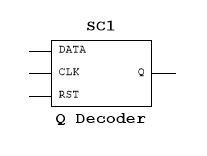
\includegraphics[width=0.3\linewidth]{images/q_idea.PNG}
        \caption{Schemat ideowy automatu wykrywającego kod Morse'a litery Q
        w strumieniu danych.}
        \label{fig:q_idea}
    \end{figure}

    \subsection{Rozwiązanie teoretyczne}
    Podany problem można rozwiązać stosująć automat Moore'a lub automat Mealy'ego.
    Ponieważ zależy nam na łatwości testowania zastosujemy automat Moore'a, którego wyjście jest funkcją wyłącznie stanu wewnętrzengo.

    Rozwiązanie zadania należy zacząć od zdefiniowania automatu deterministycznego nad alfabetem $ A =  \{a, b\} $, który znajdzie się w stanie akceptującym po otrzymaniu sekwencji $ 1101 $.
    
    Konstrujemy najprostrzy, częściowo uzupełniony automat akceptujący $1101$ i patrzymy czy da się go uzupełnić aby działał dla dłuższych sekwencji.

    \begin{figure}[h!] 
        \centering 
        \begin{tikzpicture}
            \node[state, initial] (A) {$A$};
            \node[state, right of=A] (B) {$B$};
            \node[state, right of=B] (C) {$C$};
            \node[state, right of=C] (D) {$D$};
            \node[state, accepting, right of=D] (E) {$E$};
            \draw 
                (A) edge[bend left, above] node{1} (B)
                (B) edge[bend left, above] node{1} (C)
                (C) edge[bend left, above] node{0} (D)
                (D) edge[bend left, above] node{1} (E);
        \end{tikzpicture}
        \caption{Pierwsza propozycja automatu}
        \label{fig:simple_automata}
    \end{figure}

    Uzupełniamy krawędzie tak aby powstał pełny deterministyczny automat skończony.

    \begin{figure}[H] 
        \centering 
        \begin{tikzpicture}
            \node[state, initial] (A) {$A$};
            \node[state, right of=A] (B) {$B$};
            \node[state, right of=B] (C) {$C$};
            \node[state, right of=C] (D) {$D$};
            \node[state, accepting, right of=D] (E) {$E$};
            \draw 
                (A) edge[loop above] node{0} (A)
                (A) edge[bend left, above] node{1} (B)
                (B) edge[bend left, above] node{1} (C)
                (B) edge[bend left, above] node{0} (A)
                (C) edge[loop above] node{1} (C)
                (C) edge[bend left, above] node{0} (D)
                (D) edge[bend left, above] node{1} (E)
                (D) edge[bend left, above] node{0} (A)
                (E) edge[bend left, above] node{0} (A)
                (E) edge[bend left, above] node{1} (C);
        \end{tikzpicture}
        \caption{Ostateczny schemat automatu}
        \label{fig:complex_automata}
    \end{figure}

    % TODO czy można to jakoś uzasadnić na tym etapie że automat jest ok, oprócz tego że "na logikę"

    W celu przniesienia logiki autmatu na przerzutniki D definujemy tabelę przejść.
    Do każdego stanu przydzielamy trzybitową nazwę zgodnie z kodem Graya aby nie trzeba było później zamieniać ich kolejności przy wpisywaniu do tabeli Karnaugh.
    Odpowiednio $ A \to  000 $, $ B \to  001$, $ C \to 011$, $ D \to 010$, $ E \to 110$.

    \begin{table}[!htb]
        \begin{minipage}{.5\linewidth}
            \centering
            \begin{tabular}{|c | c | c |} 
            \hline
            Stan & \multicolumn{2}{c|}{Wejście}\\
            \hline
            $Q_{2}Q_{1}Q_{0}$ & 0 & 1 \\ 
            \hline
            \hline
            000(A) & 000(A) & 001(B) \\
            \hline
            001(B) & 000(A) & 011(C) \\
            \hline
            011(C) & 010(D) & 011(C) \\
            \hline
            010(D) & 000(A) & 110(E) \\
            \hline
            110(E) & 000(A) & 011(C) \\
            \hline
            111 & X & X\\
            \hline
            101 & X & X\\
            \hline
            100 & X & X \\
            \hline
            \end{tabular}
            \caption{Tabela przejść automatu}
        \end{minipage}%
        \begin{minipage}{.5\linewidth}
            \centering
            \begin{tabular}{|c | c |} 
            \hline
            Stan & Wejście\\
            \hline
            $Q_{2}Q_{1}Q_{0}$ & 0 \\ 
            \hline
            \hline
            000(A) & 0 \\
            \hline
            001(B) & 0 \\
            \hline
            011(C) & 0 \\
            \hline
            010(D) & 0 \\
            \hline
            110(E) & 1 \\
            \hline
            111 & X \\
            \hline
            101 & X \\
            \hline
            100 & X \\
            \hline
            \end{tabular}
            \caption{Tabela akceptacji automatu}
        \end{minipage} 
    \end{table}

    Trzy ostatnie stany pozostawiamy niezdefiniowane.
    \begin{figure}[H]
        \begin{minipage}{.5\linewidth}
            \begin{karnaugh-map}[4][4][1][$Q_{0}X$][$Q_{2}Q_{1}$]
                \manualterms{0, 1, 0, 1, 0, 0, 0, 1, X, X, X, X, 0, 1, X, X}
                \implicant{1}{11}
                \implicant{4}{5}
            \end{karnaugh-map}
            \caption{D0}
        \end{minipage}
        \begin{minipage}{.5\linewidth}
            \begin{karnaugh-map}[4][4][1][$Q_{0}X$][$Q_{2}Q_{1}$]
                \manualterms{0,0,0,1,0,1,1,1,X,X,X,X,0,1,X,X}
                \implicant{3}{7}
                \implicant{5}{13}
                \implicant{6}{14}
            \end{karnaugh-map}
            \caption{D1}
        \end{minipage}
        \begin{minipage}{1\linewidth}
            \centering
            \begin{karnaugh-map}[4][4][1][$Q_{0}X$][$Q_{2}Q_{1}$]
                \manualterms{0,0,0,0,0,1,0,0,X,X,X,X,0,0,X,X}
                \implicant{5}{5}
            \end{karnaugh-map}
            \caption{D2}
        \end{minipage}
    \end{figure}

    Z powyższych tabel można odczytać wzory które pozwolą na zbudowanie układu.

    \begin{align*} 
        D_{0} &=  \color{red}{X} \color{green}\overline{(\overline{Q_{2}}Q_{1}\overline{Q_{0}})} \color{black}= X (Q_{2}+\overline{Q_{1}}+Q_{0}) \\ 
        D_{1} &=  {\color{green}\overline{Q_0} X Q_{1}} + {\color{olive}\overline{X}Q_0Q_1}+{\color{red}\overline{Q_2}Q_0X}\\
        D_{2} &= {\color{red}Q_{0}XQ_{1}\overline{Q_{2}}} \\
        Y &= Q_{2}
    \end{align*}

    \subsection{Wprowadzanie danych}
    Wprowadzanie danych do urządzenia można obsłużyć przy pomocy dwóch
    szyn: szyny danych i szyny zegara. Przycisk "kropka" ustawia stan wysoki
    na szynie zegara, a "kreska" - zarówno na zegarze, jak i na danych.
    W ten sposób układ pracuje niezależnie od odstępów między kolejnymi naciśnięciami
    przycisków.

    \begin{figure}[h]
        \centering
        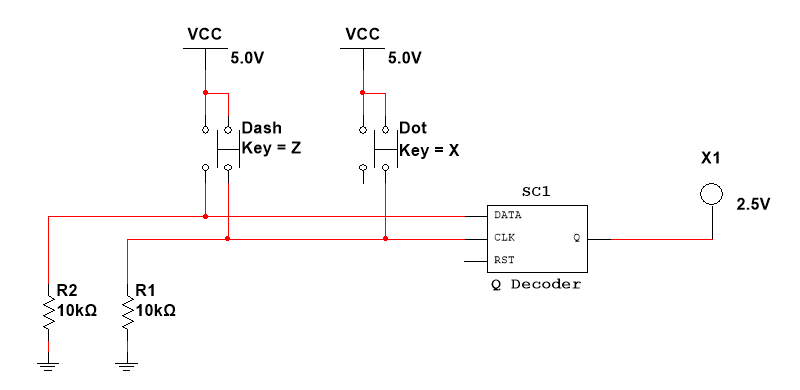
\includegraphics[width=\linewidth]{images/q_input.PNG}
        \caption{Schemat układu pozwalającego wprowadzać dane do automatu}
        \label{fig:q_input}
    \end{figure}


    \begin{figure}[h]
        \centering
        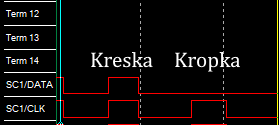
\includegraphics[width=0.3\linewidth]{images/q_input_plot.PNG}
        \caption{Wykres stanów szyn danych i czasu podczas wprowadzania
        sygnału}
        \label{fig:q_idea_plot}
    \end{figure}

    \subsection{Projektowanie układu}

    Wzory wyznaczone wyżej
    \begin{align*} 
        D_{0} &=  X \overline{(\overline{Q_{2}}Q_{1}\overline{Q_{0}})} = X (Q_{2}+\overline{Q_{1}}+Q_{0}) \\ 
        D_{1} &=  \overline{Q_0} X Q_{1} + \overline{X}Q_0Q_1+\overline{Q_2}Q_0X\\
        D_{2} &= Q_{0}XQ_{1}\overline{Q_{2}} \\
        Y &= Q_{2}
    \end{align*}

    \begin{figure}[H]
        \centering
        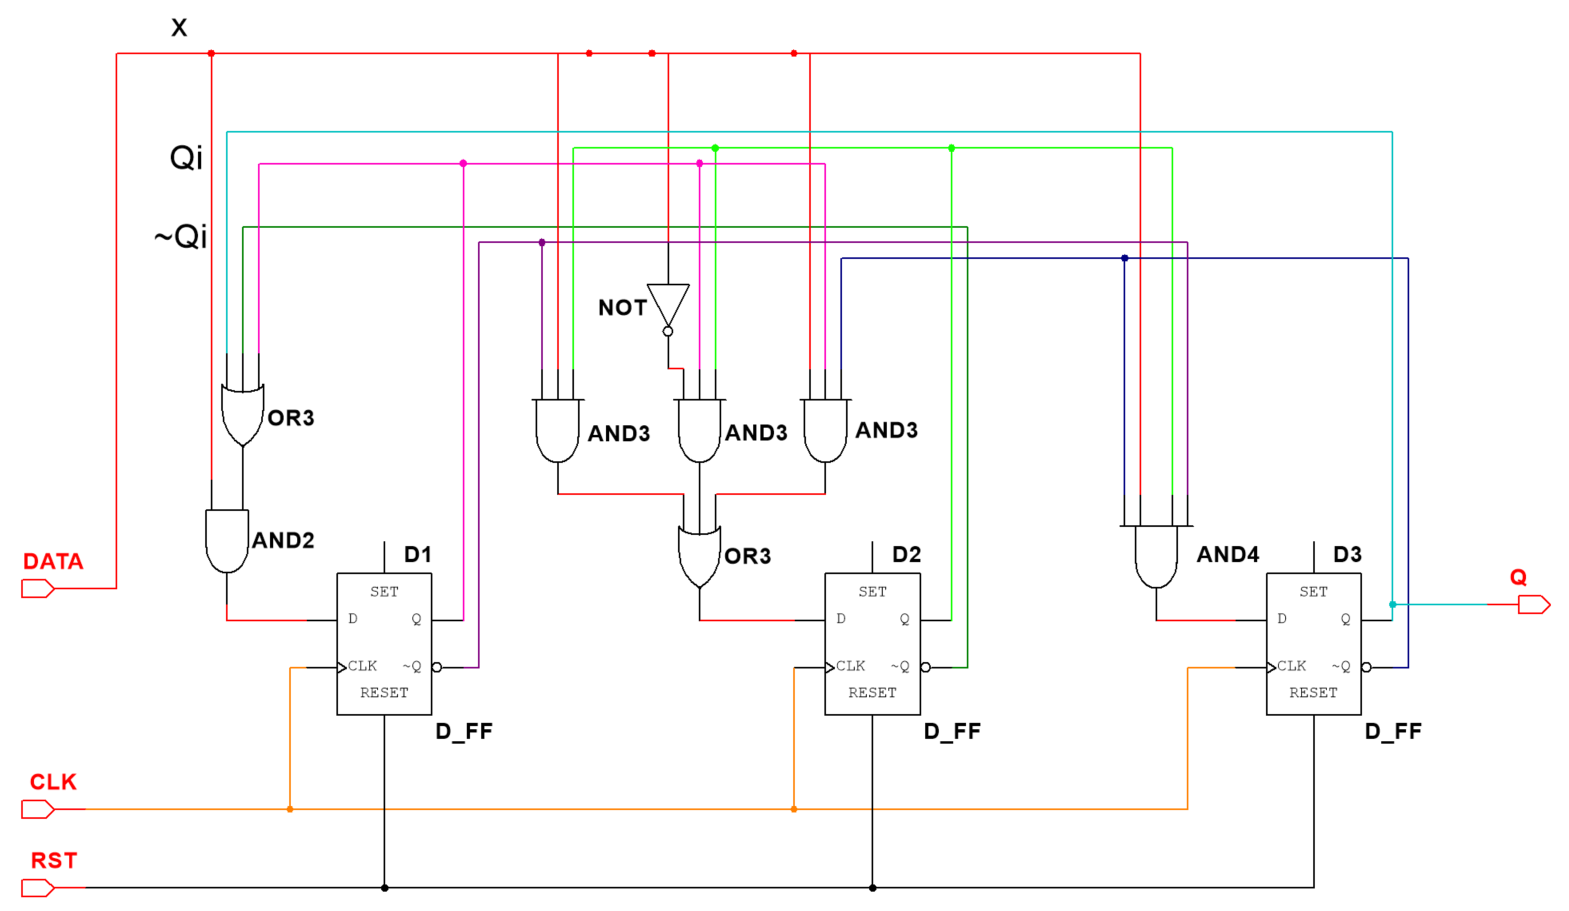
\includegraphics[width=1.0\linewidth]{images/3c_schematic.png}
        \caption{Schemat układu}
    \end{figure}

    W układnie korzystamy z trzech przerzutników D.
    Sposób podłączenia można bezpośrednio wywnioskować ze wzoru.
    Wzór na $ D_i $ mówi co należy podłączyć do wejścia $d$ przerzutnika $i$.
    $Q_i$ to wartość wyjścia $q$ przerzutnika $i$. 
    Wyjście układu należy podłączyć od wyjścia ostatniego przerzutnika.
    Piny zegara łączymy ze spólnym pinem zegara układu.

    W celu dodania możliwości prostego resetowania układu do stanu początkowego łączymy
    piny reset na przerzutnikach z pinem resetowania układu.


    \subsection{Wnioski}
    \begin{enumerate}
        \item Istnieją różne sposoby wprowadzania danych. 
        Zdecydowaliśmy się na dwa przyciski odpowiadające kropce i kresce, czego skutkiem jest konieczność opóźniania sygnału aby wyjście się ustabilizowało.
        Alternatywnie można było użyć dwóch przełączników, gdzie jeden odpowiada za dane a drugi potwierdza wprowadzenie.
        Takie rozwiązanie pomimo że skutkuje prostrzym układem jest mało intuicyjne w użytkowaniu.
        \item Opóźnienie można najprościej zaimplementować szeregowo połączonymi bramkami które razem nie modyfikuja wartości logicznej.
        Bardziej typowym rozwiązaniem jest zastosowanie opóźnienia w oparciu o układ RC, kosztem większego skomplikowania schematu.
    \end{enumerate}

    \subsection{Zastosowania}
    \begin{enumerate}
        \item Pokazany układ wykrywa sekwencje odpowiadającą literze Q w alfabecie Morse'a.
        Po skonstruowaniu w analogiczny sposób układów dla każdej litery można zbudowac urządzenie, które tłumaczy wiadomość.
        \begin{figure}[H]
            \centering
            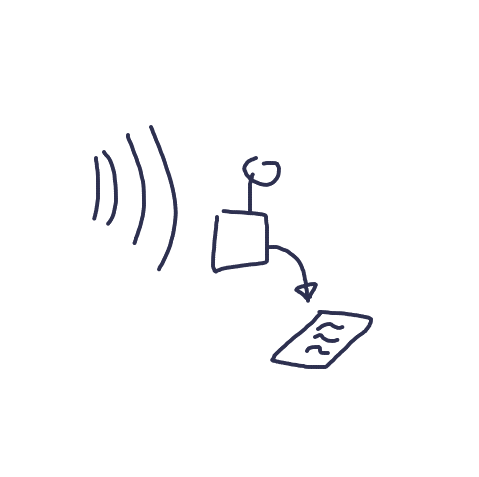
\includegraphics[width=0.3\linewidth]{images/translate.png}
            \caption{Tłumacznie wiadomości z alfabetu Morse'a}
        \end{figure}
        \item Można zmodyfikować układ aby wykrywał sekwencję odpowiadającą SOS i zbudować urządzenie, które
        po podpięciu do radia może włączać alarm kiedy ktoś nada taki sygnał.
        \begin{figure}[H]
            \centering
            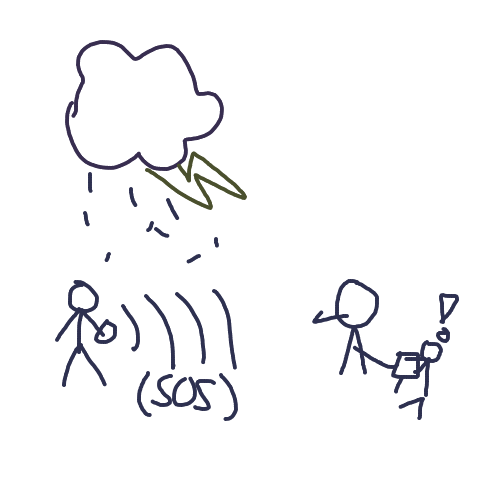
\includegraphics[width=0.3\linewidth]{images/sos.png}
            \caption{Wykrywanie sygnału SOS}
        \end{figure}
        \item Można układ połączyć z dzwonkiem do drzwi i elektronicznym zamkiem, 
        który umożliwia otworzenie drzwi jedynie osobom które znają sekwencję.
        translate
        \begin{figure}[H]
            \centering
            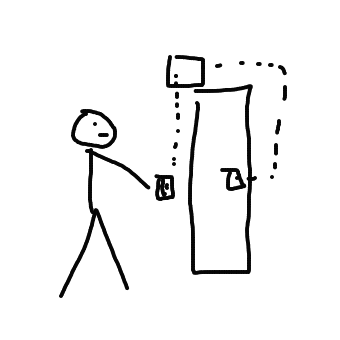
\includegraphics[width=0.3\linewidth]{images/door.png}
            \caption{Zamek otwierający drzwi po wprowadzeniu sekwencji}
        \end{figure}
    \end{enumerate}
\end{document}